\section{Ejercicio 4}

Consideremos el siguiente lote de tareas, que usaremos para corroborar el funcionamiento del scheduler \textbf{Round Robin}:

\begin{minipage}[t]{0.3\textwidth}
\begin{tarea}[H]
\begin{verbatim}
@1:
TaskCPU 6
TaskCPU 5
@3:
TaskCPU 1
\end{verbatim}\end{tarea}
\end{minipage}\\\\

En este lote se puede apreciar que las dos primeras tareas se agregarán a la cola ready global en el mismo momento (en el tiempo 1), pero respetando el orden de entrada a dicha cola. Luego una tercera tarea se agregará a la cola ready en el tiempo 3. Como puede observarse, todas las tareas son de tipo \texttt{TaskCPU}, ya que no realizan IO.

Ejecutando este lote en un procesador de un único núcleo, con un \textit{quantum} $= 3$ y cambio de contexto $= 0$ obtenemos el comportamiento dado por el siguiente diagrama de Gantt:

%\FloatBarrier

\begin{figure}[h!t]
  \centering
  \makebox[\textwidth][c]{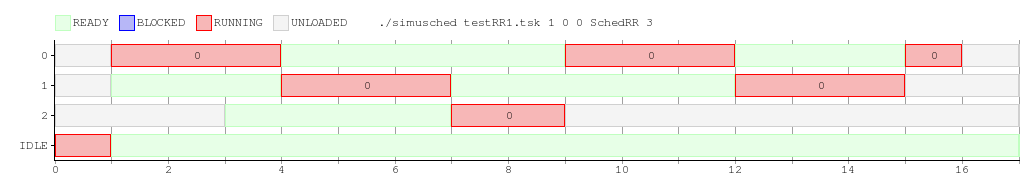
\includegraphics[width=1.2\textwidth]{graphics/ej4-01.png}}%
  \caption{Lote de 3 tareas ejecutándose en \textbf{Round Robin}}
  \label{fig:fig41}
\end{figure}

La tarea \texttt{IDLE} comienza ejecutándose ya que no se encuentra ninguna tarea en la ready queue en el tiempo 0. La tarea 0 (de duración 6) comienza a ejecutarse ni bien entra en la ready queue en el tiempo 1. La misma se ejecuta por 3 ticks (la duración del \textit{quantum}), hasta que es desalojada en favor de la tarea 1. Esta misma también se ejecuta por 3 ticks hasta que es desalojada a su vez en favor de la tarea 2. Como la duración de esta tarea es de 2 ticks (1 tick de duración sumado al tick de terminación) esto hace que se cambie la tarea a ejecutar nuevamente por la 0 antes de la finalización de su \textit{quantum}. Finalizado el \textit{quantum} de la tarea 0 se cambia a la tarea 1, la cual consume todo su \textit{quantum} y termina (por ser de duración 5). Por último, se ejecuta el tick de terminación de la tarea 1 y el procesador queda entonces sin carga.

Al haberse utilizado un único núcleo, se observa claramente cómo el mismo distribuye su tiempo entre las distintas tareas de forma circular (según el orden de la cola), concediendo a cada una de ellas una cantidad uniforme de ticks igual al valor del \textit{quantum}. Dadas estas características, y el hecho de que las tareas se ejecutan sin distinción de prioridad, el scheduler efectivamente muestra comportamiento tipo \textbf{Round Robin}.